\documentclass[
  bibliography=totoc,     % Literatur im Inhaltsverzeichnis
  captions=tableheading,  % Tabellenüberschriften
  titlepage=firstiscover, % Titelseite ist Deckblatt
]{scrartcl}

% Paket float verbessern
\usepackage{scrhack}

% Warnung, falls nochmal kompiliert werden muss
\usepackage[aux]{rerunfilecheck}

% unverzichtbare Mathe-Befehle
\usepackage{amsmath}
% viele Mathe-Symbole
\usepackage{amssymb}
% Erweiterungen für amsmath
\usepackage{mathtools}

% Fonteinstellungen
\usepackage{fontspec}
% Latin Modern Fonts werden automatisch geladen
% Alternativ zum Beispiel:
%\setromanfont{Libertinus Serif}
%\setsansfont{Libertinus Sans}
%\setmonofont{Libertinus Mono}

% Wenn man andere Schriftarten gesetzt hat,
% sollte man das Seiten-Layout neu berechnen lassen
\recalctypearea{}

% deutsche Spracheinstellungen
\usepackage{polyglossia}
\setmainlanguage{german}


\usepackage[
  math-style=ISO,    % ┐
  bold-style=ISO,    % │
  sans-style=italic, % │ ISO-Standard folgen
  nabla=upright,     % │
  partial=upright,   % ┘
  warnings-off={           % ┐
    mathtools-colon,       % │ unnötige Warnungen ausschalten
    mathtools-overbracket, % │
  },                       % ┘
]{unicode-math}

% traditionelle Fonts für Mathematik
\setmathfont{Latin Modern Math}
% Alternativ zum Beispiel:
%\setmathfont{Libertinus Math}

\setmathfont{XITS Math}[range={scr, bfscr}]
\setmathfont{XITS Math}[range={cal, bfcal}, StylisticSet=1]

% Zahlen und Einheiten
\usepackage[
  locale=DE,                   % deutsche Einstellungen
  separate-uncertainty=true,   % immer Fehler mit \pm
  per-mode=symbol-or-fraction, % / in inline math, fraction in display math
]{siunitx}

% chemische Formeln
\usepackage[
  version=4,
  math-greek=default, % ┐ mit unicode-math zusammenarbeiten
  text-greek=default, % ┘
]{mhchem}

% richtige Anführungszeichen
\usepackage[autostyle]{csquotes}

% schöne Brüche im Text
\usepackage{xfrac}

% Standardplatzierung für Floats einstellen
\usepackage{float}
\floatplacement{figure}{htbp}
\floatplacement{table}{htbp}

% Floats innerhalb einer Section halten
\usepackage[
  section, % Floats innerhalb der Section halten
  below,   % unterhalb der Section aber auf der selben Seite ist ok
]{placeins}

% Seite drehen für breite Tabellen: landscape Umgebung
\usepackage{pdflscape}

% Captions schöner machen.
\usepackage[
  labelfont=bf,        % Tabelle x: Abbildung y: ist jetzt fett
  font=small,          % Schrift etwas kleiner als Dokument
  width=0.9\textwidth, % maximale Breite einer Caption schmaler
]{caption}
% subfigure, subtable, subref
\usepackage{subcaption}

% Grafiken können eingebunden werden
\usepackage{graphicx}
% größere Variation von Dateinamen möglich
\usepackage{grffile}

% schöne Tabellen
\usepackage{booktabs}

% Verbesserungen am Schriftbild
\usepackage{microtype}

% Literaturverzeichnis
\usepackage[
  backend=biber,
]{biblatex}
% Quellendatenbank
\addbibresource{lit.bib}
\addbibresource{programme.bib}

% Hyperlinks im Dokument
\usepackage[
  unicode,        % Unicode in PDF-Attributen erlauben
  pdfusetitle,    % Titel, Autoren und Datum als PDF-Attribute
  pdfcreator={},  % ┐ PDF-Attribute säubern
  pdfproducer={}, % ┘
]{hyperref}
% erweiterte Bookmarks im PDF
\usepackage{bookmark}

% Trennung von Wörtern mit Strichen
\usepackage[shortcuts]{extdash}

\usepackage{subcaption}

\author{%
  Jannis Speer\\%
  \href{mailto:jannis.speer@tu-dortmund.de}{jannis.speer@tu-dortmund.de}%
  \texorpdfstring{\and}{,}%
  Kevin Talits\\%
  \href{mailto:kevin.talits@tu-dortmund.de}{kevin.talits@tu-dortmund.de}%
}
\publishers{TU Dortmund – Fakultät Physik}

\setlength{\parindent}{0 pt}

\subject{V402}
\title{Dispersionsmessung am Glasprisma}
\date{%
  Durchführung: 19.06.2018
  \hspace{3em}
  Abgabe: 26.06.2018
}

\begin{document}

\maketitle
\thispagestyle{empty}
\tableofcontents
\newpage

\section{Einleitung}

Beim Übergang von einem Medium in ein anderes erfährt eine Lichtwelle eine Richtungsänderung
aufgrund der materialabhängigen Ausbreitungsgeschwindigkeit.
Dieser Effekt wird als Brechung bezeichnet und kann mit dem Huygenschen Prinzip erklärt werden.
Zur Beschreibung der Brechung wird der Brechungsindex benutzt, der als das Verhältnis
der Ausbreitungsgeschwindigkeiten der zwei Mediens definiert ist.
Da die Ausbreitungsgeschwindigkeit von der Frequenz bzw. der Wellenlänge abhängt,
besteht für den Brechungsindex eine Dispersionsrelation,
die über eine Dispersionskurve beschrieben wird.
\begin{equation*}
  n = f(\lambda)
\end{equation*}
Im Experiment soll nun die Dispersionskurve eines Glasmaterials
über die Untersuchung der zweifachen Brechung eines Lichtstrahls beim Durchgang durch ein Prisma untersucht werden.

\section{Theorie}
\label{sec:Theorie}
Als Spannungsquelle wird hier ein Gerät verwedet, welches über einen endlichen Zeitraum hinweg eine konstante elektrische Leistung liefert.
Für die Kenntnis über das Verhalten der Spannungsquelle innerhalb einer elektrischen Schaltung, müssen die Leerlaufspannung und der Innenwiderstand bekannt sein.
Genau dann, wenn der Spannungsquelle kein Strom entnommen wird, liegt an ihr die Leerlaufspannung $U_0$ an.
Wenn ein endlicher Strom $\symbf{I}$ durch einen Lastwiderstnd $R_a$ fließt, sinkt die Spannung $U_k$, welche an den Ausgangsbuchsen der belasteten Spannungsquelle abgegriffen werden kann, unter $U_0$.
Durch die Zuordnung eines Innenwiderstandes $R_i$ zur Spannungsquelle kann dieses Phänomen formal erklärt werden.
Die Maschenregel besagt: \enquote{Die Summe aller Spannungsabfälle an den Widerständen $R_m$ der Masche ist gleich die Summe der Leerlaufspnnungen.}, daraus folgt also:
\begin{equation}
  \sum_{n} U_{0_n} = \sum_{m} R_m \symbf{I}_m
  \label{eqn:eq1}
\end{equation}
Nach Abb. \ref{fig:abb1} folgt mit $U_{0_n} = U_0$, $\symbf{I}_m = \symbf{I}$ für $m = 1, 2$, $R_1 = R_i$ und $R_2 = R_a$ die Gleichung
\begin{equation}
  U_0 = \symbf{I} R_i + \symbf{I} R_a
  \label{eqn:eq2}
\end{equation}
\begin{figure}
  \centering
  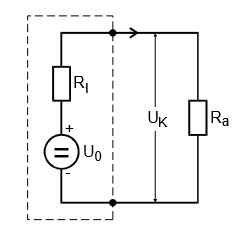
\includegraphics{data/abb1.jpg}
  \caption{Ersatzschaltbild einer realen Spannungsquelle mit Lastwiderstand $R_a$. \cite{V301}}
  \label{fig:abb1}
\end{figure}
\FloatBarrier
\noindent
Für $U_k$ ergibt sich dann
\begin{equation}
  U_k = \symbf{I} R_a = U_0 - \symbf{I} R_i
  \label{eqn:eq3}
\end{equation}
Daraus folgt das Absinken der Spannung $U_k$ mit zunehmenden Strom.
Durch ein hochohmiges Voltmeter und dem dadurch sehr geringen Strom beim Messen der Leerlaufspannung kann das Glied $\symbf{I} R_i$ in Gleichung \ref{eqn:eq3} vernachlässigt werden.
So gilt $U_k \approx U_0$.
Der umrandete Teil in Abb. \ref{fig:abb1} wird Ersatzschaltbild einer realen Spannungsquelle genannt.
Durch idealisierte Bauteile, deren Wirkungsweise bekannt ist, wird das elektrische Verhalten eines realen Objekts beschrieben.
Für eine reale Spannungsquelle wird der ohmsche Widerstand $R_i$ und eine dazu in Reihe geschaltete ideale Spannungsquelle benötigt.
Diese ist ideal, weil sie eine von äußeren Einflüssen unabhängige Spannung $U_0$ bei einem Innenwiderstand von null liefert.
Durch $R_i$ kann einer Spannungsquelle auch keine beliebig hohe elektrische Leistung entnommen werden.
Die an $R_a$ abgegebene Leistung $N = \symbf{I}^2 R_a$ durchläuft ein Maximum.
Ist $R_a$ so groß gewählt, dass N maximal wird, wird von Leistungsanpassung gesprochen.
Der Innenwiderstand elektrischer Generatorn ist nicht zwingend durch den Gleichstromwiderstand gegeben, sondern beispielsweise durch einen Rückkopplungsmechanismus.
Somit ist es von Nöten den Innenwiderstand als differentielle Größe einzuführen.
\begin{equation}
  R_i = \frac{dU_k}{d\symbf{I}}
  \label{eqn:eq4}
\end{equation}

\section{Durchführung}
\label{sec:Durchführung}

\subsection{Versuche im elektrischen Feld}

Im ersten Versuchsteil (siehe Abb \ref{fig:V1}) wird für 5 verschiedene Beschleunigungsspannungen $U_\text{B}$ zwischen 180 und 500 V die Verschiebung des Leuchtflecks in Abhängigkeit der Ablenkspannung $U_\text{d}$ untersucht.
Dafür wird die Ablenkspannung so eingestellt, dass der Leuchtfleck nacheinander auf den 9 äquidistanten Linien des Koordinatennetzes liegt.
\begin{figure}
  \centering
  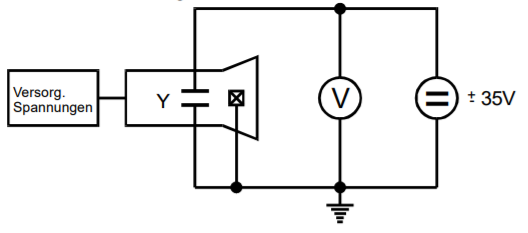
\includegraphics{data/V1.png}
  \caption{Schaltung für Ablenkung im elektischen Feld.}
  \label{fig:V1}
\end{figure}

Im zweiten Versuchsteil wird ein Oszillograph nach Abbildung \ref{fig:V2} aufgebaut.
\begin{figure}
  \centering
  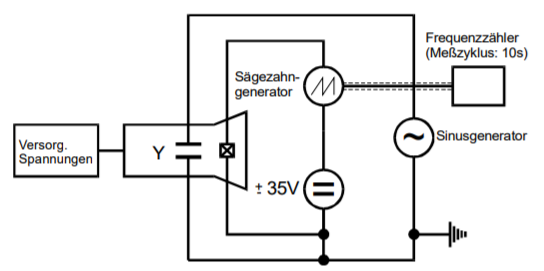
\includegraphics{data/V2.png}
  \caption{Schaltung für Oszillographen.}
  \label{fig:V2}
\end{figure}
Die Freqeunz einer Sinusspannung soll über Regulation der Sägezahnfrequenz bestimmt werden, die wie in Kapitel \ref{sec:Oszillograph} im rationalen Verhältnis zur Sinusfrequenz steht, wenn das Bild der Sinusspannung auf dem Bildschirm steht.
Außerdem soll die Amplitude der Sinusspannung über die maximale Strahlauslenkung bestimmt werden.
Für diese Berechnung muss die Beschleunigungsspannung bekannt sein.

\subsection{Versuch im magnetischen Feld}

Die spezifische Ladung der Elektronen wir mit Hilfe eines Elektronenstrahls gemessen, der durch das nahezu homogene Feld einer Helmholtz-Spule auf eine Kreisbahn abgelenkt wird.
Die Kathodenstrahlröhre wird unter Verwendung eines Deklinatorium-Inklinatorium parallel zur Horizontalkomponente des Magnetfelds ausgerichtet.
Für eine konstante Beschleunigungsspannung von 250 und 500 V wird die Abhängigkeit von $B$, das über die Spannung an den Spulen reguleirt wird und $D$, das an den Linien des Leuchtschirms abgelesen wird, untersucht.

In Nord-Süd-Richtung wirkt auf den Elektronenstrahl keine Kraft, die vom Erdmagnetfeld ausgeht, im Gegensatz zur Ost-West-Richtung.
Das Magnetfeld der Helmholtz wird so eingestellt, dass sich beide Magnetfelder gegenseitig aufheben.
Daraus kann die Größe der Horizontalkomponente des ErdMagnetfelds geschlossen werden.
Um die Totalintensität des Erdmagnetfeldes $B_\text{total}$ zu bestimmen, wird mit Hilfe des Inklinatoriums der Winkel zwischen Horizontalebene und Richtung des Erdmagnetfeldes (Inklinationswinkel) bestimmt.

\section{Auswertung}
\label{sec:Auswertung}
Die notierten Werte lauten:
\begin{align}
L = (10.11 +/- 0.03) mH
C = (2.098 +/- 0.006) nF
R_1 = (48.1 +/- 0.1) \si{\ohm}
R_2 = (509.5 +/- 0.5) \si{\ohm}
\end{align}
Die gemessenen Daten der Spannungsamplitude $U_c$ und dazugehöriger Zeiten $t$,
befinden sich im Anhang auf Tabelle 1.
Der angefertigte Plot der Einhüllenden des Abklingvorgangs ist in \ref{fig:plot1} zu sehen.
\begin{figure}
  \centering
  \includegraphics{build/plot1.pdf}
  \caption{Abklingvorgang des gedämpften RCL-Schwingkreises mit Fit.}
  \label{fig:plot1}
\end{figure}

Die Form der Einhüllenden nach \eqref{eqn:gl7} ist gegeben durch:
\begin{equation}
  A = A_0 e^(-2 \pi \mu t)
\end{equation}
Mit der Ausgleichsrechnung ergeben sich die Werte:
\begin{align}
  A_0 = (224.58 +/- 4.29) \si{\volt}
  \mu = (261 +/- 16) \frac{1}{s}
\end{align}
Daraus ergeben sich nach \eqref{eqn:gl8} und $T_ex = \frac{1}{2 \pi \mu}$ die Werte für den Effektivwiderstand $R_{\text{eff}}$ und die Abklingdauer $T_{\text{ex}}$:
\begin{align}
  R_{\text{eff}} = (33.2 +/- 2.0) \si{\ohm}
  T_{\text{ex}} = (0.61 +/- 0.4) ms
\end{align}
Der in der Schaltung verbaute Widerstand$R_1 = (48.1 +/- 0.1) \si{\ohm}$ weicht um $14.9 \si{\ohm}$ ab.
Der gemessene Wert für $R_ap$, bei dem der aperiodische Grenzfall eintritt, beträgt $3280 \si{\ohm}$.
Verglichen mit dem durch $\frac{1}{LC} = \frac{(R_ap)^2}{4L^2}$ berechneten Wert von $(4390 +/- 9) \si{\ohm}$, zeigt sich eine Differenz von $1110 \si{\ohm}$.
Dies ist zum Einen dadurch zu erklären, dass die restlichen Bauteile, vor allem die Spule, ebenfalls in der Theorie nicht beachtete Widerstände haben.
Zum anderen konnte ein genaues Einstellen nicht erfüllt werden, da im Bereich um den Grenzwiderstand keine wesentliche Änderung am Spannungsverlauf zu erkennen waren.

Die gemessenen Daten zur Bestimmung der Resonanzüberhöhung $q$, sowie der Breite der Resonanzkurve $\nu_+ - \nu_-$ befinden sich im Anhang in Tabelle 2.
Die Erregerspannung $U$ beträgt dabei $117 \si{\volt}$.
Deren Frequenzabhängigkeit ist nach experimentellem Nachweis am Oszilloskop vernachlässigbar.
Das Verhältnis $\frac{U_c}{U}$ wird gegen $f$ , zu sehen in \ref{fig:plot2}, abgetragen.
Der Maximalwert $q_exp$ wird aus dem Graphen als Güte abgelesen.

\begin{figure}
  \centering
  \includegraphics{build/plot2.pdf}
  \caption{Normierte Kondenstorspannung in Abhängigkeit von der Frequenz.}
  \label{fig:plot2}
\end{figure}

Wird der theoretische Wert der Güte nach $q = \frac{1}{\omega_o R C}$ bestimmt, so ergibt sich:
\begin{align}
  q_exp = 2.45
  q_theo = 3.923 +/- 0.009
  \intertext{relative Abweichung:}
  \frac{q_theo - q_exp}{q_theo} = 37.5 \%
\end{align}
Um die Breite der Resonanzkurve bestimmen zu können, wird der Frequenzbereich um das Maximum nun linear dargestellt.
Das Ergebnis is in \ref{fig:plot3} zu sehen.
Aus dieser wird die Breite der Resonanzkurve abgelesen und die Werte werden mit den durch $\omega_+ - \omega_- \approx \frac{R}{L}$ theoretisch berechneten Werten verglichen:
\begin{align}
  \intertext{Experimentell:}
  \nu_+ - \nu_- = 11140 Hz
  \intertext{Theoretisch:}
  \nu_+ - \nu_- =
  \intertext{relaive Abweichung:}
\end{align}

\begin{figure}
  \centering
  \includegraphics{build/plot3.pdf}
  \caption{Lineare Darstellung der normierten Kondenstorspannung in Abhängigkeit von der Frequenz.}
  \label{fig:plot3}
\end{figure}

Die Messdaten, um die Werte für die Resonanzfrequenz $\nu_res$, sowie für die Frequenzen $\nu_1$ beziehungsweise $\nu_2$, an denen die Phase $\frac{\pi}{4}$ beziehungsweise $\frac{3 \pi}{4}$ beträgt,
berechnen zukönnen, befinden sich im Anhang in Tabelle 3. Die Phase $\Phi$ wird in \ref{fig:plot4} gegen die Frequenz abgetragen.
Der Bereich um die Resonanzfrequenz wird, wie in \ref{fig:plot4} erkennbar, zur besseren Ablesbarkeit linear dargestellt.
$\nu_res$ wird nach $ \omega_res = \sqrt{\frac{1}{LC} - \frac{R^2}{2L^2}}$ und $\nu_1$ und $\nu_2$ werden nach $\omega_(1,2) = +/- \frac{R}{2L} + \sqrt{\frac{R^2}{4L^2} + \frac{1}{LC}}$ errechnet und mit den abgelesenen Werten verglichen:

\begin{align}
  \nu_(res, exp) = 33 000 Hz
  \nu_(res, theo) = (34 280 +/- 70) Hz
  \intertext{relative Abweichung:}
  3.7 \%
  \nu_(1, exp) = 27 200 Hz
  \nu_(1, theo) =(30 430 +/- 60) Hz
  \intertext{relative Abweichung:}
  10.6 \%
  \nu_(2, exp) = 38 340 Hz
  \nu_(2, theo) = (39 240 +/- 80) Hz
  \intertext{relative Abweichung:}
  2.3 \%
\end{align}

\begin{figure}
  \centering
  \includegraphics{build/plot4.pdf}
  \caption{Lineare Darstellung der Phasenverschiebung zwischen Kondensator- und Erregerspannung.}
  \label{fig:plot4}
\end{figure}

\section{Diskussion}
\label{sec:Diskussion}

Durch den nicht unendlich dünn auflösbaren Leuchtpunkt sind exakte Messungen der Ablenkung nicht möglich.
Diese Ungenauigkeit konnte lediglich durch Fokusierung des Punktes verkleinert, aber nicht eliminiert werden.
Bei der Messung der Ausrichtung des Ermagnetfeldes und des Inklinationswinkels gab es Ungenauigkeit durch die Schwerfälligkeit des Deklintoriums.
Die Drehachsen waren zu schwergängig um jedes Mal zuverlässige Ergebnisse zu liefern.
Nur mit sehr viel feingefühl sind akzeptable Werte zu vermessen.
Die Abweichungen der Ergebisse liegen noch im akzeptablen bereich, bis auf die spezifische Ladung von Elektronen.
Diese imense Abweichung liegt entweder an Fehlern bei der Messung oder zu ungenauen Werten.
Die Frequenz der Sinusspannung ist als gut zu schätzen, weil am Sinusgenerator zum Vergleich ein ungefähres Frequenzspektrum von 80-90 Hz angegeben war.
Die errechneten 79.92 Hz liegen nah genug am Spektrum um realistisch zu sein.

\printbibliography{}

\end{document}
